\documentclass[a4paper,10pt]{article}
\usepackage{tueposter2018}
\usepackage[english]{babel}
\usepackage{graphicx}
\usepackage{booktabs}
\usepackage{tikz}
\usepackage{pgfplots}
\pgfplotsset{compat=1.18}
\usepackage{titlesec}
\titlespacing*{\section}{0pt}{1.5ex plus 0.3ex minus 0.2ex}{0.8ex plus 0.1ex}

\title{Testing Medical VLM Generalization on Rare Cases}
\subtitle{MedGemma, BiomedCLIP, and MedSigLIP on Open-MELON}
\authors{Daan Merx, Domas Berulis, Roma den Otter}
\department{Department of Biomedical Engineering}

\begin{document}
\maketitle

\begin{multicols}{2}

%%% COLUMN 1 %%%

\section*{Abstract}
How well do medical VLMs generalize to rare histopathology cases? We evaluate whether caption-based MedGemma can classify melanoma vs.\ nevus on 913 Open-MELON histopathology images, and benchmark it against embedding-based classifiers (BiomedCLIP, MedSigLIP).

\section*{Methodology}
\textbf{Dataset.} Open-MELON-VL-2.5K~[1]: 913~samples (597~melanoma, 316~benign). Ground truth labelling by keyword matching.

\noindent\textbf{Caption cleaning.} Original captions contain non-visual metadata (staining, magnification, citations). Gemini rewrites each caption to retain only visual pathology and diagnosis, producing cleaned references for labeling and RAGAS evaluation.

\noindent\textbf{Generative.} MedGemma-1.5-4B-it~[2] (Q4\_K\_M). Caption generation. Caption quality scored via RAGAS~[5] (Gemini-judged faithfulness and relevance vs.\ cleaned references). 4~prompts $\times$ 3~decoding settings (deterministic, mild sampling at $T{=}0.2$, moderate sampling at $T{=}0.5$).

\noindent\textbf{Embeddings.} BiomedCLIP~[3] (512-d) and MedSigLIP~[4] (768-d) with LogReg, SVM, Random Forest.

\noindent\textbf{Evaluation.} Each trial samples equal numbers per class. We report balanced accuracy averaged over 10~trials. Failure theme analysis on shared hard cases.

%%% COLUMN 2 %%%

\section*{Main Results}

\begin{center}
\begin{tikzpicture}
\begin{axis}[
    ybar, bar width=5pt,
    width=\linewidth, height=4.5cm,
    ylabel={Balanced Acc.\ (\%)},
    ylabel style={font=\scriptsize},
    ymin=40, ymax=82, ytick={40,50,60,70,80},
    y tick label style={font=\tiny},
    symbolic x coords={MedGemma, {BC+LR}, {BC+SVM}, {BC+RF}, {MS+LR}, {MS+SVM}, {MS+RF}},
    xtick=data,
    x tick label style={rotate=35, anchor=east, font=\tiny},
    nodes near coords,
    every node near coord/.append style={font=\tiny, /pgf/number format/fixed, /pgf/number format/precision=1},
    error bars/y dir=both,
    error bars/y explicit,
    enlarge x limits=0.12,
]
\addplot+[fill=tuescarlet!80, draw=tuescarlet] coordinates {
    (MedGemma, 50.6) +- (0, 3.0)
    ({BC+LR}, 73.1) +- (0, 3.0)
    ({BC+SVM}, 73.9) +- (0, 2.9)
    ({BC+RF}, 72.6) +- (0, 2.5)
    ({MS+LR}, 71.4) +- (0, 4.1)
    ({MS+SVM}, 74.0) +- (0, 3.3)
    ({MS+RF}, 71.6) +- (0, 5.2)
};
\end{axis}
\end{tikzpicture}%
\vspace{-0.9em}
\captionof{figure}{Balanced accuracy (10 trials). BC\,=\,BiomedCLIP, MS\,=\,MedSigLIP.}
\end{center}

\noindent\textbf{MedGemma bias.} Binary-choice prompt: 99.4\% melanoma recall but only 0.7\% nevus recall. The model predicts melanoma for nearly every sample. Balanced accuracy: 50.6\%.

\noindent\textbf{Caption quality.} The open prompt scores 0.15 faithfulness / 0.23 relevance; the binary-choice prompt improves to 0.44 / 0.57, but still indicates only partial alignment with reference pathology.

\begin{center}
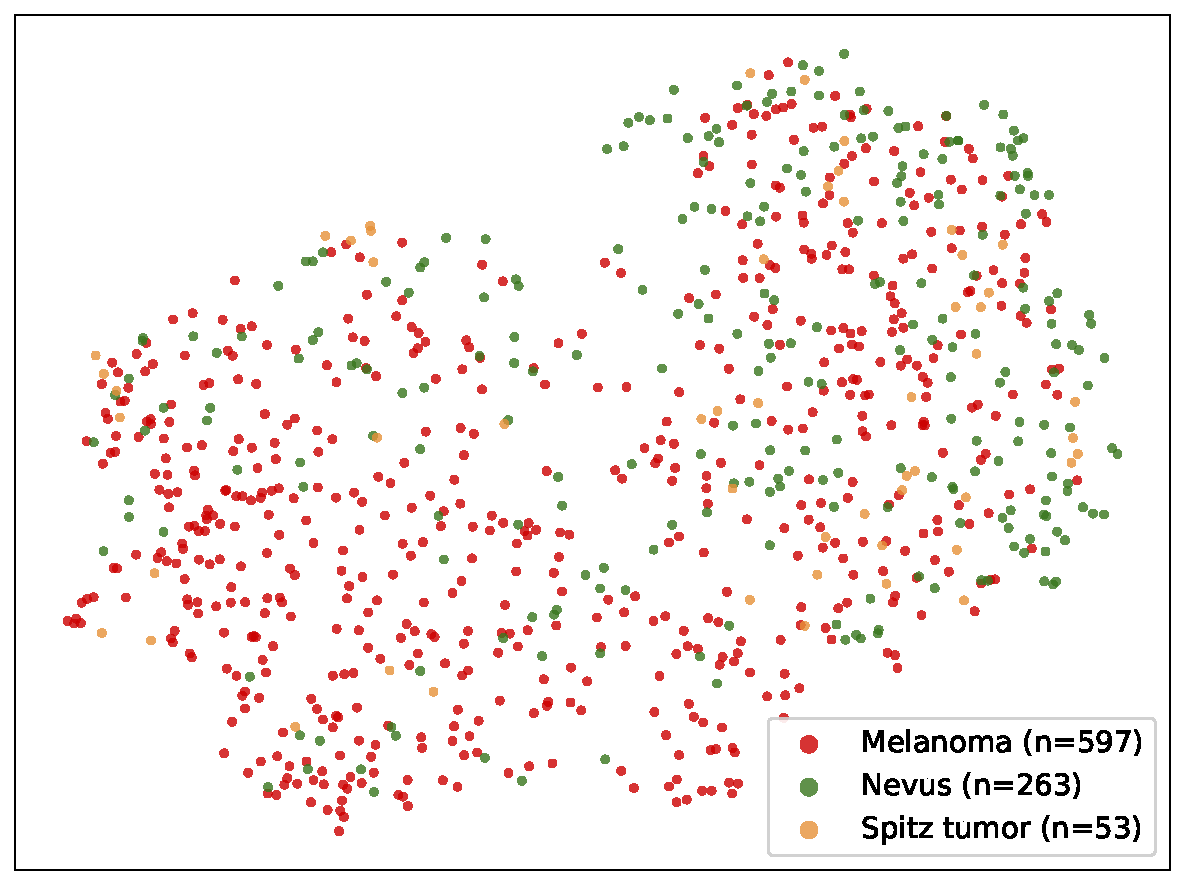
\includegraphics[width=\linewidth]{umap_medsiglip.pdf}
\vspace{-0.9em}
\captionof{figure}{UMAP projection of MedSigLIP embeddings. Some separation between nevus and melanoma clusters is visible, but far from clean. Spitz tumor embeddings scatter across melanoma-dense regions, showing their features are indistinguishable from melanoma.}
\end{center}

%%% COLUMN 3 %%%

\section*{Discussion}
\begin{itemize}\setlength{\itemsep}{1pt}\setlength{\parskip}{0pt}
\item MedGemma fails to generalize: melanoma bias persists across all prompt configurations tested.
\item We identified 35 cases where both BiomedCLIP and MedSigLIP SVMs fail. These concentrate in diagnostically challenging subtypes from both directions: benign lesions that mimic malignancy (Spitz tumors, cellular blue nevi) and melanomas that defy typical appearance (in-situ, mucosal, desmoplastic). These are cases that challenge even expert dermatopathologists, suggesting the models have reached a performance ceiling set by genuine morphological ambiguity.
\item Labels extracted by Gemini from caption text, not from expert pathologist annotation, label noise is possible.
\end{itemize}

\section*{Conclusion}
\fbox{\parbox{0.92\linewidth}{\centering\small\bfseries%
MedGemma does not generalize well. It overcalls melanoma on benign lesions regardless of prompt, prioritizing sensitivity over specificity.}}

\begin{thebibliography}{9}
{\small
\bibitem{openmelon} Han et al.\ (2024). Open-MELON-VL-2.5K.
\bibitem{medgemma} Google (2024). MedGemma.
\bibitem{biomedclip} Zhang et al.\ (2023). BiomedCLIP. \textit{arXiv:2303.00915}.
\bibitem{medsiglip} Hamamci et al.\ (2024). MedSigLIP.
\bibitem{ragas} Es et al.\ (2023). RAGAS. \textit{arXiv:2309.15217}.
}
\end{thebibliography}

\end{multicols}
\end{document}
